\documentclass[t]{beamer}
\usetheme{Copenhagen}
\setbeamertemplate{headline}{} % remove toc from headers
\beamertemplatenavigationsymbolsempty

\usepackage{amsmath, array, tikz, bm, pgfplots, tcolorbox, graphicx, venndiagram, color, colortbl, xfrac}
\pgfplotsset{compat = 1.16}
\usepgfplotslibrary{statistics}
\usetikzlibrary{calc}

\title{Other Probability Distributions}
\author{}
\date{}

\AtBeginSection[]
{
  \begin{frame}
    \frametitle{Objectives}
    \tableofcontents[currentsection]
  \end{frame}
}

\begin{document}

\begin{frame} 
\maketitle
\end{frame}

\section{Solve problems involving geometric probability distributions}

\begin{frame}{Binomial vs. Geometric Distributions}
With binomial distributions, we had the following conditions:
	\begin{itemize}
		\item There are a fixed number of $n$ repeated independent trials
		\item Each trial's outcome is either a success or failure
		\item The probability of success, $p$, never changes
	\end{itemize}	
	\vspace{10pt}
\onslide<2->{We could calculate the probability of obtaining 8 heads out of 10 flips of a coin.}	\newline\\
\onslide<3->{One of these outcomes is TTHTHHHTTH.}	
\end{frame}

\begin{frame}{Binomial vs. Geometric Distributions}
With geometric distributions, we would interested in the probability of obtaining our first success (flipping a tail) after $x$ flips of the coin.	\newline\\	
\onslide<2->{To put it another way, a geometric distribution has the following property:}
\onslide<3->{\[\underbrace{FFF \cdots F}_{x-1 \text{ failures}}S\]}
\end{frame}

\begin{frame}{Geometric Distributions}
The probability of obtaining our first success after $x$ binomial experiments is given by
\[P(X=x) = (1-p)^{x-1} \cdot p\]
\end{frame}

\begin{frame}{Example 1}
A student is given a 10-question multiple choice test in which each question has 5 possible answers. What is the probability that the first question the student guesses correctly on the 4th question?	\newline\\

FFFS	

\begin{align*}
P(X = 4) &= (1-0.2)^4 (0.2)	\\
&= 0.08192
\end{align*}
\end{frame}

\begin{frame}{Bar Graph of Example 1}
\begin{center}
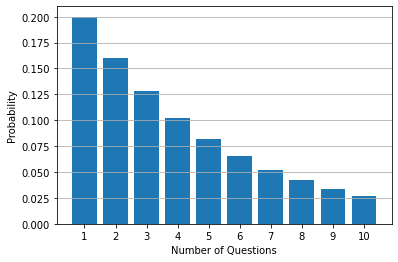
\includegraphics[scale=0.6]{../Images/geometric_mult_choice.png}
\end{center}
\end{frame}

\begin{frame}{Mean and Standard Deviation of Geometric Distributions}
The mean (expected value) of a geometric distribution is the {\color{blue}\textbf{reciprocal of the probability of success}}:

\[E(X) = \frac{1}{p}\]

\pause
The variance for a geometric distribution is the probability of failure divided by the square of the probability of success, given as 
\[\sigma^2 = \frac{1-p}{p^2}\]
\pause

From which the standard deviation, $\sigma$ is
\[\sigma = \sqrt{\frac{1-p}{p^2}} = \frac{\sqrt{1-p}}{p}\]

\end{frame}

\begin{frame}{Example 2}
(a)	\quad A student is given a 10-question multiple choice test in which each question has 5 possible answers. What is the expected number of answers a student can guess before getting one right?	\newline\\	\pause

The expected value is the reciprocal of the probability of success:
\begin{align*}
\onslide<3->{E(X) &= \frac{1}{0.2}} \\[10pt]
\onslide<4->{&= 5} 
\end{align*}

\onslide<5->{We would expect the student to answer 5 questions before guessing one correctly.}
\end{frame}

\begin{frame}{Example 2}
(b) \quad What is the standard deviation of the number of questions needed before the student guesses correctly?	\newline\\	\pause

The standard deviation is the square root of the probability of failue divided by the probability of success:
\begin{align*}
\onslide<3->{\sigma &= \frac{\sqrt{1-0.2}}{0.2}} \\[8pt]
\onslide<4->{& \approx 4.47}
\end{align*}

\onslide<5->{The standard deviation is about 4.47 questions.}
\end{frame}

\section{Solve problems involving hypergeometric probability distributions}


% Hypergeometric Distributions
% Poisson Distributions

\end{document}